\documentclass{standalone}

% graphics
\usepackage{tikz}
\usepackage{pgfplots}
\usepackage{siunitx}

\begin{document}

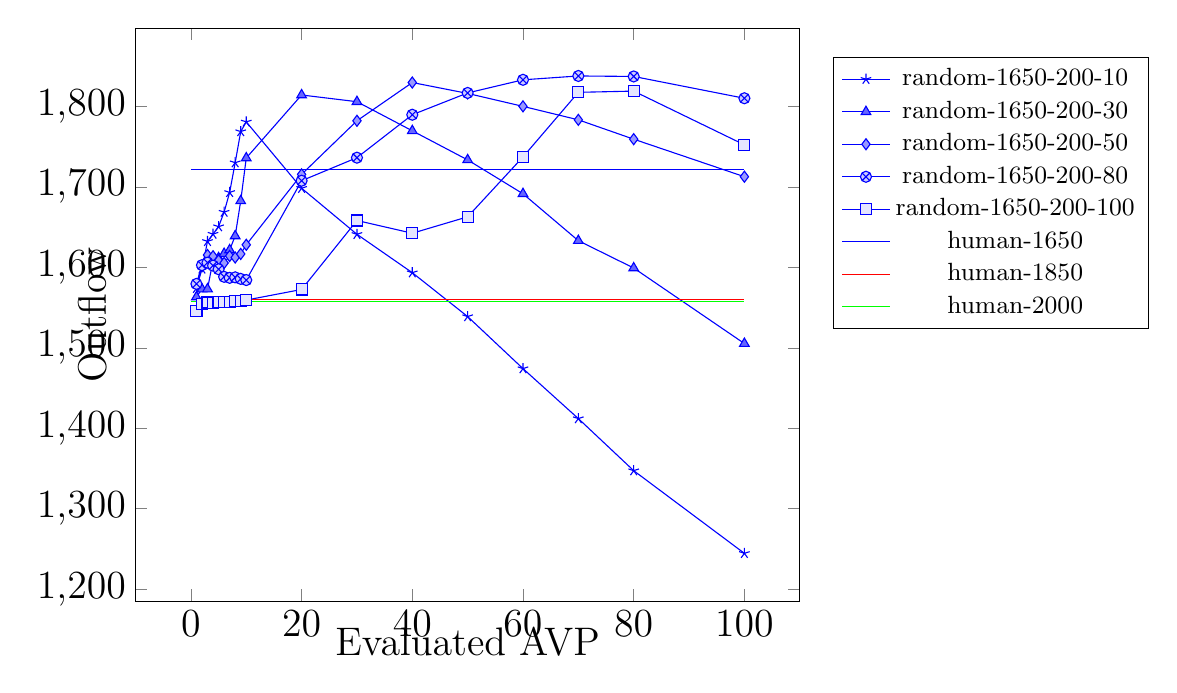
\begin{tikzpicture}[scale=1]
  \pgfplotsset{
      scale only axis,
      every x tick label/.append style={font=\Large},
      every y tick label/.append style={font=\Large},
	legend style={at={(1.05,0.95)},anchor=north west}
  }

\pgfplotscreateplotcyclelist{mycolorlist}{%
	blue,every mark/.append style={fill=blue!80}, mark=star, error bars/.cd, y dir=both, y explicit\\%
	blue,every mark/.append style={fill=blue!60}, mark=triangle*, error bars/.cd, y dir=both, y explicit\\%
	blue,every mark/.append style={fill=blue!40}, mark=diamond*, error bars/.cd, y dir=both, y explicit\\%
	blue,every mark/.append style={fill=blue!20}, mark=otimes*, error bars/.cd, y dir=both, y explicit\\%
	blue,every mark/.append style={fill=blue!10}, mark=square*, error bars/.cd, y dir=both, y explicit\\%
	red,densely dashed,every mark/.append style={solid,fill=red!80}, mark=star, error bars/.cd, y dir=both, y explicit\\%
	red,densely dashed,every mark/.append style={solid,fill=red!60},mark=triangle*, error bars/.cd, y dir=both, y explicit\\%
	red,densely dashed,every mark/.append style={solid,fill=red!40},mark=diamond*, error bars/.cd, y dir=both, y explicit\\%
	red,densely dashed,every mark/.append style={solid,fill=red!20}, mark=otimes*, error bars/.cd, y dir=both, y explicit\\%
	red,densely dashed,every mark/.append style={solid,fill=red!10}, mark=square*, error bars/.cd, y dir=both, y explicit\\%
	green!40!black, dashed,every mark/.append style={solid,fill=green!80}, mark=star, error bars/.cd, y dir=both, y explicit\\%
	green!40!black, dashed,every mark/.append style={solid,fill=green!60},mark=triangle*, error bars/.cd, y dir=both, y explicit\\%
	green!40!black, dashed,every mark/.append style={solid,fill=green!40},mark=diamond*, error bars/.cd, y dir=both, y explicit\\%
	green!40!black, dashed,every mark/.append style={solid,fill=green!20},mark=otimes*, error bars/.cd, y dir=both, y explicit\\%
	green!40!black, dashed,every mark/.append style={solid,fill=green!10},mark=square*, error bars/.cd, y dir=both, y explicit\\%
	black, dashed,every mark/.append style={solid,fill=green!80}, mark=star, error bars/.cd, y dir=both, y explicit\\%
	black, dashed,every mark/.append style={solid,fill=green!60},mark=triangle*, error bars/.cd, y dir=both, y explicit\\%
	black, dashed,every mark/.append style={solid,fill=green!40},mark=diamond*, error bars/.cd, y dir=both, y explicit\\%
	black, dashed,every mark/.append style={solid,fill=green!20},mark=otimes*, error bars/.cd, y dir=both, y explicit\\%
	black, dashed,every mark/.append style={solid,fill=green!10},mark=square*, error bars/.cd, y dir=both, y explicit\\%
	}


\begin{axis}[
    legend style={font=\small},
	ylabel={\Large Outflow},
	x label style={at={(axis description cs:0.5,-0.03)},anchor=north},
	y label style={at={(axis description cs:-0.030,0.5)}, anchor=south},
	xlabel={\Large Evaluated AVP},
	cycle list name=mycolorlist
]

\addplot table [x=a, y=b] {
a	 b	 c
1	1574.03	17.33
2	1598.04	19.58
3	1632.38	22.39
4	1641.38	20.9
5	1650.67	24.6
6	1668.74	25.46
7	1693.22	27.09
8	1730.16	33.72
9	1768.86	34.18
10	1780.88	35.2
20	1698.41	39.87
30	1641.13	46.69
40	1593.4	55.7
50	1538.86	61.6
60	1474.16	69.98
70	1412.03	84.56
80	1347.3	90.21
100	1244.52	97.85
};
\label{random-1650-200-10}

\addplot table [x=a, y=b] {
a	 b	 c
1	1563.16	15.05
2	1573.09	16.57
3	1573.09	17.28
4	1608.73	19.73
5	1611.86	21.24
6	1617.16	19.83
7	1621.69	22.19
8	1639.08	29.47
9	1682.64	38.17
10	1735.96	37.0
20	1814.33	41.29
30	1805.98	33.97
40	1769.8	30.57
50	1733.62	34.44
60	1691.53	35.17
70	1633.21	38.76
80	1599.23	45.89
100	1505.34	57.09
};
\label{random-1650-200-30}

\addplot table [x=a, y=b] {
a	 b	 c
1	1578.64	15.1
2	1601.39	15.48
3	1615.43	18.22
4	1613.84	16.22
5	1608.66	17.38
6	1605.46	18.22
7	1614.17	18.84
8	1612.26	23.21
9	1616.72	27.41
10	1628.1	28.24
20	1715.65	39.88
30	1782.25	44.09
40	1829.81	40.72
50	1816.27	33.17
60	1800.18	28.49
70	1783.44	27.85
80	1759.39	24.09
100	1712.74	27.0
};
\label{random-1650-200-50}

\addplot table [x=a, y=b] {
a	 b	 c
1	1579.5	17.38
2	1602.79	14.3
3	1605.92	14.63
4	1602.18	17.06
5	1597.68	17.36
6	1588.28	15.8
7	1586.99	18.48
8	1587.64	20.31
9	1585.73	17.92
10	1584.25	22.83
20	1707.73	26.92
30	1736.39	46.23
40	1789.78	49.27
50	1816.88	46.87
60	1833.19	41.14
70	1837.98	31.18
80	1837.37	29.54
100	1810.26	25.74
};
\label{random-1650-200-80}

\addplot table [x=a, y=b] {
a	 b	 c
1	1545.52	20.24
2	1554.84	15.96
3	1556.35	15.48
4	1556.17	13.97
5	1557.22	14.98
6	1557.36	15.49
7	1557.47	13.69
8	1557.76	14.12
9	1557.9	14.66
10	1559.38	14.95
20	1572.55	21.39
30	1658.3	21.78
40	1642.46	28.68
50	1662.88	40.11
60	1737.32	48.93
70	1817.64	48.09
80	1819.15	28.01
100	1752.37	21.87
};
\label{random-1650-200-100}

\addplot[blue, samples=200] coordinates {(0,1722.200000) (100,1722.200000)};\label{human-1650}\addplot[red, samples=200] coordinates {(0,1560.380000) (100,1560.380000)};\label{human-1850}\addplot[green, samples=200] coordinates {(0,1558.120000) (100,1558.120000)};\label{human-2000}\addlegendimage{/pgfplots/refstyle=random-1650-200-10}
\addlegendentry{random-1650-200-10}
\addlegendimage{/pgfplots/refstyle=random-1650-200-30}
\addlegendentry{random-1650-200-30}
\addlegendimage{/pgfplots/refstyle=random-1650-200-50}
\addlegendentry{random-1650-200-50}
\addlegendimage{/pgfplots/refstyle=random-1650-200-80}
\addlegendentry{random-1650-200-80}
\addlegendimage{/pgfplots/refstyle=random-1650-200-100}
\addlegendentry{random-1650-200-100}
\addlegendimage{/pgfplots/refstyle=human-1650}
\addlegendentry{human-1650}
\addlegendimage{/pgfplots/refstyle=human-1850}
\addlegendentry{human-1850}
\addlegendimage{/pgfplots/refstyle=human-2000}
\addlegendentry{human-2000}


\end{axis}
\end{tikzpicture}
\end{document}
